\documentclass[11pt,class=report,crop=false]{standalone}
\usepackage[screen]{../python}



\begin{document}

%====================================================================
\chapitre{Compléments d'arithmétique}
%====================================================================

\insertvideo{lTRK4CEh7nc}{partie 14.1. Fractions continues}

\insertvideo{7m2HBBf8QPw}{partie 14.2. Algorithme de Shor pour n'importe quel ordre}

\insertvideo{OWanCeO3Hqo}{partie 14.3. L'algorithme de Shor fonctionne au moins une fois sur deux}


\objectifs{Nous apportons des compléments à l'algorithme de Shor vu lors du chapitre précédent en étudiant chacune des hypothèses.}

\bigskip


\objectifs{Dans ce chapitre il n'y a pas d'informatique quantique mais beaucoup de mathématiques ! Certaines parties sont assez techniques et d'un niveau un peu plus élevé que les chapitres précédents.}


%%%%%%%%%%%%%%%%%%%%%%%%%%%%%%%%%%%%%%%%%%%%%%%%%%%%%%%%%%%%%%%%%%%%%
\section{Fractions continues}

\index{fraction continue}

%--------------------------------------------------------------------
\subsection{Motivation}

Dans le chapitre précédent nous avons fait une hypothèse simplificatrice : l'ordre $r$ divise $2^n$. Ce n'est pas vrai en général, mais l'algorithme de Shor reste valide moyennant quelques adaptations.


Reprenons la fin du circuit de l'algorithme de Shor qui permet de calculer l'ordre $r$ d'un élément.
\begin{itemize}
  \item Si $r$ divise $2^n$ alors la mesure du premier registre conduit à un nombre rationnel $x = \frac{m}{2^n}$ qui est aussi égal à $\frac{\ell}{r}$.
  Ainsi $x$ est un multiple de $\frac 1r$ et permet de retrouver $r$ (ou au moins un facteur de $r$).
   
  \item Si $r$ ne divise pas $2^n$ alors la mesure du premier registre conduit à un nombre rationnel $x = \frac{m}{2^n}$ qui est proche d'un multiple de $\frac1r$ (mais n'est pas exactement un multiple). Comment retrouver $r$ à partir de $x$ ?
\end{itemize}


Voici l'exemple que l'on étudiera en détails dans la section suivante afin de factoriser
$N=21$ à l'aide du choix $a=2$. 
Imaginons qu'une mesure conduise à $x = \frac{427}{512}$. Comment retrouver l'ordre $r$ ? On pourrait aussi obtenir $x = \frac{426}{512}$ ou bien $x = \frac{428}{512}$.
On voit que $x$ est proche de $\frac45$. Mais est-ce que $5$ est vraiment la période ? 

%--------------------------------------------------------------------
\subsection{Fractions continues}


Une \defi{fraction continue} est une fraction 
$$a_0 + \frac{1}{a_1 + \frac{1}{a_2+\frac{1}{\cdots+\frac{1}{a_n}}}}$$
où $a_0\ge0$ et $a_i>0$ (pour $i>0$). On note cette fraction par la liste $[a_0,a_1,\ldots,a_n]$.

On note $\frac{p_n}{q_n}$ l'écriture irréductible du rationnel $[a_0,a_1,\ldots,a_n]$.

\begin{exemple}
L'écriture en fraction continue $[5,2,1,4]$ représente le nombre rationnel :
$$x = 5 + \frac{1}{2 + \frac{1}{1 + \frac{1}{4}}} = \frac{75}{14} =  5.3571428\ldots$$

Prendre les sous-listes de la fraction continue permet d'obtenir des approximations de $x$ de plus en plus précises :
\begin{itemize}
  \item Sous liste $[5]$, alors $\frac{p_0}{q_0} = 5$.
  \item Sous liste $[5,2]$ alors $\frac{p_1}{q_1} = \frac{11}{2} = 5.5$.
  \item Sous liste $[5,2,1]$ alors $\frac{p_2}{q_2} = \frac{16}{3} = 5.33\ldots$
  \item Liste complète $[5,2,1,4]$ alors $\frac{p_3}{q_3} = \frac{75}{14} = x$.
\end{itemize}

\end{exemple}

%--------------------------------------------------------------------
\subsection{Approximations par les fractions continues}

Les fractions continues prennent tout leur intérêt pour approcher des réels (ou des rationnels) par des fractions simples.
Prenons l'exemple de $\pi$. Comment approcher $\pi$ par une fraction avec un dénominateur pas trop grand (disons avec moins de trois chiffres) ?
L'idée la plus simple est d'utiliser l'écriture décimale $\pi = 3.1415\ldots \simeq \frac{314}{100}$. Mais peut-on faire mieux ?

Calculons pour commencer la fraction continue de $x = \frac{314}{100}$.
Cela se fait par des divisions euclidiennes successives :
$314 = 3 \times 100 + 14$ donc
$$\frac{314}{100} = 3 + \frac{14}{100} = 3 + \frac{1}{\frac{100}{14}},$$
puis $100 = 7 \times 14 + 2$, donc  
$$\frac{314}{100} = 3 + \frac{1}{7+\frac{2}{14}} = 3 + \frac{1}{7+\frac{1}{7}}.$$
Ainsi $$\frac{314}{100} \simeq 3 + \frac{1}{7} = \frac{22}{7}$$
Nous avons donc approché $\pi$ par $\frac{22}{7} = 3.1428\ldots$ ce qui est aussi bien que $\frac{314}{100}$ mais avec un dénominateur beaucoup plus petit.

Bien évidemment on peut pousser les calculs plus loin :
$\pi \simeq \frac{314\,159}{100\,000}$.
On calcule la fraction continue de $\pi$ (ou de $\frac{314\,159}{100\,000}$) et on obtient $[3, 7, 15, 1,\ldots]$. Cela fournit les approximations successives :
\begin{itemize}
  \item Sous liste $[3,7]$, alors $\frac{p_1}{q_1} = \frac{22}{7}= 3.1428\ldots$
  \item Sous liste $[3,7,15]$, alors $\frac{p_2}{q_2} = \frac{333}{106}= 3.141509\ldots$
  \item Sous liste $[3,7,15,1]$, alors $\frac{p_3}{q_3} = \frac{355}{113}= 3.14159292\ldots$
\end{itemize}

Ainsi avec des fractions dont les dénominateurs restent petits, on trouve de très bonnes approximations de $\pi$.
En un sens les fractions continues donnent les meilleures approximations possibles d'un réel $x$ par des rationnels.

%--------------------------------------------------------------------
\subsection{Exemple}

Reprenons l'exemple de la factorisation de $N=21$ à l'aide du choix $a=2$.
Supposons que le circuit de Shor nous donne la valeur $x = \frac{427}{512}$,
comment obtenir l'ordre $r$ ?

La mauvaise idée est d'utiliser l'écriture décimale pour dire $x = \frac{427}{512} \simeq \frac{400}{500} = \frac45$ donc le dénominateur naturel (qui donne l'ordre $r$) serait $5$. Ce n'est pas vrai.

La bonne méthode est de calculer le développement en fraction continue de $x$ :
$$
x 
= \frac{427}{512} 
= [0,1,5,42,2] 
= 0 + \frac{1}{1 + \frac{1}{5 + \frac{1}{42 + \frac12}}}
$$

Ce qui fournit les approximations successives :
\begin{itemize}
  \item Sous liste $[0,1] = 0+\frac11$, alors $\frac{p_1}{q_1} = \frac{1}{1} = 1$.
  \item Sous liste $[0,1,5] = 0+\frac{1}{1+\frac15}=\frac56$.
  \item Sous liste $[0,1,5,42] = 0+\frac{1}{1+\frac{1}{5+\frac1{42}}}=\frac{211}{253}$.
  \item Sous liste $[0,1,5,42,2] = \frac{427}{512}$.
\end{itemize}

Les dénominateurs sont les candidats pour l'ordre $r$, mais on sait que l'ordre $r$ cherché est inférieur à l'entier $N = 21$. Donc ici, la meilleure fraction ayant un dénominateur inférieur à $N$ est $\frac56$, on trouve ainsi $r=6$.
Il est facile de vérifier que l'ordre de $a=2$ modulo $N=21$ est bien $r=6$.


Lors de la mesure on peut aussi obtenir des valeurs légèrement différentes par exemple $x' = \frac{426}{512}$ ou bien $x'' = \frac{428}{512}$. Que se passe-t-il alors ? 
\begin{itemize}
  \item Si $x' = \frac{426}{512} = [0,1,4,1,20,2]$, les fractions successives sont $\frac11$, $\frac45$, $\frac56$, $\frac{104}{125}$, $\frac{213}{256}$. 
 La meilleure fraction ayant un dénominateur inférieur à $N$ est $\frac56$, on retrouve ainsi $r=6$.
  \item Si $x'' = \frac{428}{512} = [0,1,5,10,2]$, les fractions successives sont $\frac11$, $\frac56$, $\frac{51}{61}$, $\frac{107}{128}$. 
 La meilleure fraction ayant un dénominateur inférieur à $N$ est encore $\frac56$ et on retrouve $r=6$.
\end{itemize}

Conclusion : la méthode des fractions continues permet de retrouver l'ordre $r$.



%%%%%%%%%%%%%%%%%%%%%%%%%%%%%%%%%%%%%%%%%%%%%%%%%%%%%%%%%%%%%%%%%%%%%
\section{Algorithme de Shor pour n'importe quel ordre pair}

\index{algorithme de Shor}

%--------------------------------------------------------------------
\subsection{Fin du circuit}


\begin{itemize}
  \item \textbf{Cas du chapitre précédent.} Si $r$ divise $2^n$ alors la mesure du premier registre conduit à la mesure d'un état $\ket{\frac{2^n\ell}{r}}$ et donne donc un entier $m = \frac{2^n\ell}{r}$.  
  On définit alors le rationnel $x = \frac{m}{2^n}$ qui est aussi égal à $\frac{\ell}{r}$ et qui permet de retrouver $r$ (ou au moins un facteur de $r$).   
  Noter que comme $r$ divise $2^n$, $m$ est un multiple de $\frac{2^n}{r}$. Autrement dit, $x$ est un multiple (avec un facteur entier) de $\frac 1r$.

  \item \textbf{Cas considéré maintenant.} Si $r$ ne divise pas $2^n$ alors la mesure du premier registre conduit à un entier $m$. Cet entier $m$ est proche de $\frac{2^n\ell}{r}$ (pour un certain entier $\ell$) mais la fraction $\frac{2^n\ell}{r}$ n'est plus un entier.
  Autrement dit on obtient un nombre rationnel $x = \frac{m}{2^n}$ qui est proche d'un multiple de $\frac1r$ (mais n'est pas exactement un multiple).
\end{itemize}


%--------------------------------------------------------------------
\subsection{L'exemple $N=21$ : début}


Soit $N$ l'entier à factoriser. Dans toute la suite on considérera l'exemple de $N=21$.
Dans le cas où $r$ divise $2^n$, il suffisait de choisir l'entier $n$ tel que $N \le 2^n$. Dans le cas général on choisit $n$ de sorte à avoir les inégalités $N^2 \le 2^n < 2N^2$.
Pour $N=21$, on a $N^2 = 441$, donc avec $n=9$ on a bien $N^2 \le 2^n = 512 < 2N^2$. 

Reprenons les calculs du circuit de Shor :
\begin{itemize}
  \item \textbf{Initialisation.}
$$\ket{\psi_0} = \ket{0}^{\otimes n} \otimes \ket{0}^{\otimes n}.$$

\item \textbf{Transformation de Hadamard.} 

$$\ket{\psi_1} 
= \left(\frac{1}{\sqrt{2^n}} \sum_{k=0}^{2^n-1} \ket{\underline{k}} \right) \otimes \ket{\underline{0}}.$$

  \item \textbf{Oracle.}
  $$\ket{\psi_2} = \frac{1}{\sqrt{2^n}} \sum_{k=0}^{2^n-1} \ket{\underline{k}} \otimes \ket{\underline {a^k}}.$$
\end{itemize}


%--------------------------------------------------------------------
\subsection{L'exemple $N=21$ : milieu}

Choisissons ensuite un entier $a$ inversible modulo $N$.
Prenons simplement $a=2$ qui est bien premier avec $N=21$.
Nous devons retrouver l'ordre de $a$ modulo $N$ qui est ici $r=6$.

Réordonnons les éléments de $\ket{\psi_2}$ en regroupant les termes selon le second facteur qui est l'un des $\ket{\underline {a^k}}$ pour $k$ variant de $0$ à $r-1=5$.

\begin{align*}
\ket{\psi_2} = 
& \tfrac{1}{\sqrt{512}} \Big( \ket{\underline{0}} + \ket{\underline{6}} + \cdots + \ket{\underline{504}} + \ket{\underline{510}} \Big)  \ket{\underline 1} \\
& \tfrac{1}{\sqrt{512}} \Big( \ket{\underline{1}} + \ket{\underline{7}} + \cdots + \ket{\underline{505}} + \ket{\underline{511}} \Big)  \ket{\underline 2} \\
& \tfrac{1}{\sqrt{512}} \Big( \ket{\underline{2}} + \ket{\underline{8}} + \cdots + \ket{\underline{506}} \Big)  \ket{\underline 4} \\
& \tfrac{1}{\sqrt{512}} \Big( \ket{\underline{3}} + \ket{\underline{9}} + \cdots + \ket{\underline{507}} \Big)  \ket{\underline 8} \\
& \tfrac{1}{\sqrt{512}} \Big( \ket{\underline{4}} + \ket{\underline{10}} + \cdots + \ket{\underline{508}} \Big)  \ket{\underline{16}} \\
& \tfrac{1}{\sqrt{512}} \Big( \ket{\underline{5}} + \ket{\underline{11}} + \cdots + \ket{\underline{509}} \Big)  \ket{\underline{11}} \\
\end{align*}

Bien noter la différence avec le cas où $r$ était une puissance de $2$. Ici on n'obtient pas un tableau rectangulaire. Les deux premières lignes contiennent une somme de $86$ termes alors que les suivantes en ont seulement $85$.

On effectue ensuite une mesure du second registre et on obtient l'un des $\ket{\underline {a^k}}$. Dans la suite on suppose par exemple qu'on obtient $\ket{\underline 2}$, alors le premier registre, une fois normalisé, contient le qubit :
$$\ket{\bar \psi_3} = \tfrac{1}{\sqrt{86}} \Big( \ket{\underline{1}} + \ket{\underline{7}} + \ket{\underline{13}} +\cdots + \ket{\underline{505}} + \ket{\underline{511}} \Big).$$


%--------------------------------------------------------------------
\subsection{L'exemple $N=21$ : fin}

La dernière étape est d'appliquer la transformée de Fourier inverse et d'effectuer une mesure sur le premier registre.

\begin{align*}
\ket{\bar \psi_4}
  &= {\hat F}^{-1} \ket{\bar \psi_3} \\
  &= {\hat F}^{-1} \left( \tfrac{1}{\sqrt{86}} \sum_{\alpha=0}^{85} \ket{\underline{6\alpha + 1}} \right) \\
  &= \tfrac{1}{\sqrt{86}} 
     \sum_{\alpha=0}^{85} \tfrac{1}{\sqrt{512}} 
     \sum_{j=0}^{511} 
     e^{-2\ii \pi \frac{(6\alpha + 1)j}{512}} 
     \ket{\underline j} \\  
&=  \tfrac{1}{\sqrt{512}}
     \sum_{j=0}^{511} 
     \left(
     \tfrac{1}{\sqrt{86}}
     \sum_{\alpha=0}^{85} 
     e^{-2\ii \pi \frac{6\alpha j}{512}} 
     \right) 
     e^{-2\ii \pi \frac{j}{512}} 
     \ket{\underline j} \\   
\end{align*}

Cette fois la somme 
$$\Sigma(j) = \tfrac{1}{\sqrt{86}}
     \sum_{\alpha=0}^{85} 
     e^{-2\ii \pi \frac{6\alpha j}{512}}$$
est un nombre complexe qui peut prendre des valeurs autres que $0$ et $1$.

La mesure du premier registre conduit à la valeur $j$ avec la probabilité :
$$p_j = \tfrac{1}{512} |\Sigma(j)|^2.$$

Ces probabilités sont presque nulles sauf pour les valeurs de $j$ proches des réels
$\frac{2^n\ell}{r}$ (qui ne sont pas des entiers) avec $\ell=0,1,\ldots,r-1$.
Nous avons ici 
$$\frac{2^n}{r} = \frac{512}{6} = 85.33\ldots$$
Les valeurs $\frac{2^n\ell}{r}$ pour $\ell=0,\ldots,5$ sont les réels :
$$0 \qquad 85.33\ldots \qquad 170.66\ldots \qquad 256 \qquad 341.33\ldots \qquad 426.66\ldots$$
Donc ici les probabilités sont presque nulles, sauf autour de entiers :
$$j=0,\qquad j=85,\qquad j=171,\qquad j=256,\qquad j=341,\qquad j=427.$$

Voici le diagramme des probabilités $p_j$, pour $0 \le j < 512$. Les $6$ pics sont nettement visibles.
\begin{center}
   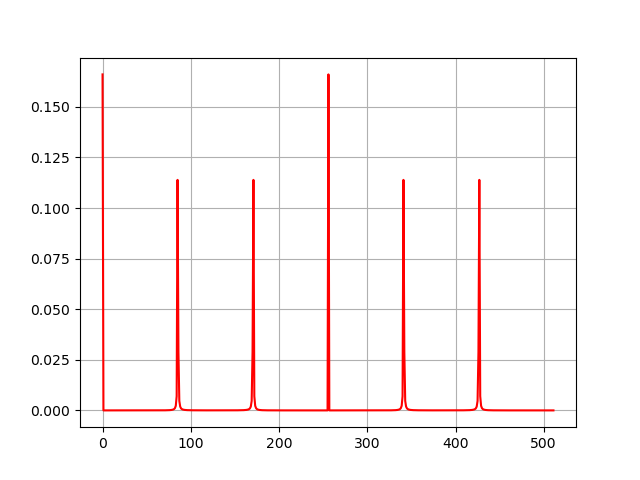
\includegraphics[scale=\myscale,scale=0.8]{figures/shor}
\end{center}
	
Voici le tableau des valeurs autour du pic à $j=427$.
$$\begin{array}{c|c}
j & p_j \\ \hline
422 &  0.00062\ldots \\
423 &  0.00099\ldots \\
424 &  0.00186\ldots \\
425 &  0.00469\ldots \\
426 &  0.02888\ldots \\
{\bf 427} &  {\bf 0.11389\ldots} \\
428 &  0.00702\ldots \\
429 &  0.00226\ldots \\
430 &  0.00109\ldots \\
431 &  0.00063\ldots \\
\end{array}
$$
On note la probabilité élevée en $j=427$, une probabilité plus faible en $j=426$
(qui s'explique car pour $\ell=5$, $\frac{2^n\ell}{r} = \frac{512\times5}{6} = 426.66\ldots$), pour les valeurs plus éloignées les probabilités sont presque nulles.

 

%--------------------------------------------------------------------
\subsection{Ordre}

On obtient l'ordre $r$, ou l'un de ses facteurs, à partir du développement en fractions continues comme expliqué précédemment. \`A part cela, les conclusions sont similaires aux cas du chapitre \og{}Algorithme de Shor\fg{} :

\begin{itemize}
  \item Si la mesure donne un entier $j$ proche de $0$, alors on n'obtient aucune information sur l'ordre $r$, il faut recommencer.
  \item Si la mesure donne un entier $j$ proche de $85$ ou proche de $427$, alors le développement en fraction continue de $\frac{j}{512}$ donne l'ordre $r=6$.
  \item Si la mesure donne un entier proche $j$ proche de $171$ ou $341$ alors on n'obtient pas $r$ mais le facteur $r'=3$ ; si la mesure donne un entier proche $j$ proche de $256$ alors on n'obtient pas $r$ mais le facteur $r''=2$. Dans ces cas on relance l'algorithme pour obtenir la factorisation complète.
\end{itemize}


%--------------------------------------------------------------------
\subsection{Conclusion}

Il nous reste à justifier que l'approximation du pic conduit au bon résultat.

\begin{theoreme}[Hardy -- Wright]
Soit $x \in \Rr$. Soit une fraction $\frac{p}{q}$ telle que :
$$\left| x - \frac{p}{q} \right| < \frac{1}{2q^2}.$$
Alors $\frac{p}{q}$ est obtenu comme l'une des fractions du développement en fractions continues de $x$.
\end{theoreme}

Dans notre situation nous considérons l'entier $m$ le plus proche de $\frac{2^n\ell}{r}$. Donc $\left|m- \frac{2^n\ell}{r}\right| \le \frac12$.
En posant $x = \frac{m}{2^n}$ on obtient $\left|x- \frac{\ell}{r}\right| \le \frac1{2^{n+1}}$.
Par notre choix de $n$ on a $2^n \ge N^2 > r^2$, donc $\left|x- \frac{\ell}{r}\right| \le \frac1{2r^2}$. Par le théorème, $\frac{\ell}{r}$ s'obtient comme l'une des fractions du développement en fractions continues de $x$, comme on l'avait expliqué dans la première section.

\bigskip

\emph{Le reste du chapitre est consacré à la théorie des groupes afin de justifier la pertinence des hypothèses 1 et 2 de l'algorithme de Shor.}

%%%%%%%%%%%%%%%%%%%%%%%%%%%%%%%%%%%%%%%%%%%%%%%%%%%%%%%%%%%%%%%%%%%%%
\section{Ordre d'un élément}

\index{groupe!ordre}

%--------------------------------------------------------------------
\subsection{Définition}

Soit $(G,\times)$ un groupe commutatif ayant pour élément neutre $e$.
L'\defi{ordre} de $x \in G$, noté $\ord(x)$, est le plus petit entier $r>0$, tel que $x^r = e$.

Voici quelques propriétés de l'ordre :
\begin{itemize}
  \item si $k$ est un entier tel que $x^k = e$ alors $\ord(x)$ divise $k$ ;
  \item $\ord(x^k)$ divise $\ord(x)$.
\end{itemize}

Le théorème de Lagrange pour un groupe fini $G$ de cardinal $n$ affirme que $x^n=e$ quel que soit $x$. Ainsi $\ord(x)$ divise $n$, quel que soit l'élément $x$. En particulier, tout élément admet un ordre fini.

%--------------------------------------------------------------------
\subsection{Plus grand ordre}

\begin{proposition}
\label{prop:maxordre}
Soit $G$ un groupe fini et $m$ le plus grand ordre parmi tous les $x \in G$,
alors pour tout $x\in G$, $\ord(x)$ divise $m$.
\end{proposition}

Une formulation équivalente est la suivante : soit $\ell$ le plus petit entier tel que pour tout $x\in G$ on ait $x^\ell = e$, alors il existe $x_0 \in G$ tel que $\ord(x_0)=\ell$.

Pour la preuve nous aurons besoin du résultat suivant :
\begin{lemme}
\label{lem:ordre}
Soient deux éléments $x$ et $y$ d'ordres $m=\ord(x)$ et $n=\ord(y)$ premiers entre eux, alors $\ord(x\cdot y) = m n$.
\end{lemme}

\begin{proof}
Notons $r=\ord(xy)$. Il s'agit de montrer $r=mn$ en prouvant que $r | mn$ puis que $mn | r$.
Tout d'abord $(xy)^{mn} = x^{mn}\cdot y^{mn} = (x^m)^n \cdot (y^n)^m = e$, donc $r | mn$.
Réciproquement, on sait que $(xy)^r=e$ donc $x^r \cdot y^r=e$, autrement dit
$z=x^r = y^{-r}$. D'une part $z^m = (x^r)^m = x^{rm} = (x^m)^r = e$, donc $\ord(z) | m$,
de même $z^n = (y^r)^n = e$, donc $\ord(z) | n$. Comme $m$ et $n$ sont premiers entre eux, alors $\ord(z)=1$, c'est-à-dire $z = e$. Ainsi $x^r=e$, donc $m=\ord(x)|r$ et
$y^r=e$ donc $n=\ord(y) | r$, ainsi $mn|r$.
\end{proof}

\begin{proof}[Preuve de la proposition]
Soit $m$ le plus grand ordre parmi les éléments de $G$,
il existe donc $y$ d'ordre $m$. 
Fixons $x$ un élément quelconque de $G$ et notons $n$ son ordre. 
Il s'agit de montrer que $n|m$.
Par l'absurde on suppose que $n$ ne divise pas $m$. 
On va obtenir une contradiction en construisant un élément $z$ avec $\ord(z)>m$.
Par exemple si $m$ et $n$ sont premiers entre eux, alors $z=xy$ est d'ordre $mn>m$, ce qui donne la contradiction.
Si $m$ et $n$ ne sont pas premiers entre eux, soit $p$ un facteur premier commun à $m$ et $n$ tel que $p^e | n$, $p^f | m$ avec $e>f$ les plus grands possibles (un tel $p$ existe car $n$ ne divise pas $m$). 
Soient $y' = y^{p^f}$ et $x' = x^{n/p^e}$. Alors  $y'$ a pour ordre $m'=m/p^f$ et $x'$ a pour ordre $n'=p^e$. Les entiers $m'$ et $n'$ sont premiers entre eux (car $m'$ n'est pas divisible par $p$). Ainsi $z=x'y'$ a pour ordre $m'n' = \frac{m}{p^f} p^e = m p^{e-f} > m$. On obtient bien la contradiction cherchée.
\end{proof}


%%%%%%%%%%%%%%%%%%%%%%%%%%%%%%%%%%%%%%%%%%%%%%%%%%%%%%%%%%%%%%%%%%%%%
\section{Le groupe $(\Zz/p\Zz)^*$}

Dans toute la suite nous allons étudier en détails le groupe $(\Zz/n\Zz)^*$ qui est l'ensemble des éléments inversibles modulo $n$. 
Nous commençons par le cas d'un nombre premier $p$.
Nous savons déjà que 
$$\Card (\Zz/p\Zz)^* = \varphi(p) = p-1$$ mais nous souhaitons aller plus loin en étudiant la structure de $(\Zz/p\Zz)^*$.

%--------------------------------------------------------------------
\subsection{Isomorphisme}

\begin{theoreme}
\label{th:zp}
Le groupe $\big((\Zz/p\Zz)^*,\times\big)$ est isomorphe au groupe $\big(\Zz/(p-1)\Zz,+\big)$.
\end{theoreme}

Pour la preuve nous aurons besoin du résultat suivant.
\begin{proposition}
\label{prop:degre}
Un polynôme $P \in \Zz/p\Zz[X]$ de degré $d$ possède au plus $d$ racines, c'est-à-dire des éléments $x\in\Zz/p\Zz$ tels que $P(x) \equiv 0 \pmod p$.
\end{proposition}


\begin{proof}[Idée de la preuve de la proposition]
C'est un fait général : sur un corps $k$ un polynôme $P \in k[X]$ de degré $d$ a au plus $d$ racines. En effet, $a \in k$ est une racine si et seulement si $X-a$ est un facteur de $P(X)$. Si $\{a_1,\ldots,a_k\}$ est l'ensemble des racines de $P(X)$ alors 
$(X-a_1)(X-a_2)\cdots(X-a_k)$ divise $P(X)$ et donc en comparant les degrés : $\deg P \ge k$.
\end{proof}

\begin{proof}[Preuve du théorème]
L'ensemble $(\Zz/p\Zz)^* = \{1,2,\ldots,p-1\}$ est en bijection avec $\Zz/(p-1)\Zz
= \{0,1\ldots,p-2\}$.
Mais on veut plus : on veut que les structures de groupes, avec la loi \og{}$\times$\fg{} pour  $(\Zz/p\Zz)^*$ et \og{}$+$\fg{} pour $\Zz/(p-1)\Zz$, soient  préservées.
Nous allons trouver un élément $a$ d'ordre $p-1$ dans $(\Zz/p\Zz)^*$ ce qui va nous permettre de construire l'isomorphisme :
$$
\begin{array}{cccc}
\phi : & \Zz/(p-1)\Zz & \longrightarrow & (\Zz/p\Zz)^* \\
       & k            &\longmapsto      & a^k \pmod p.
\end{array}
$$
Cette application $\phi$ est bien définie car $\phi(k+\ell(p-1))= a^{k+\ell(p-1)} = a^k = \phi(k)$ et est un morphisme car $\phi(k+k') = \phi(k) \times \phi(k')$. De plus $\phi$ est bijective, car elle est surjective (puisque les $\{a^k\}$ sont $p-1$ éléments distincts, ils forment l'ensemble d'arrivée) et les ensembles de départ et d'arrivée ont le même nombre d'éléments.

Pour montrer qu'il existe un élément d'ordre $p-1$, remarquons d'abord que pour tout élément $x \in (\Zz/p\Zz)^*$ on a $\ord(x) | p-1$.
En effet, par le petit théorème de Fermat, $x^{p-1} \equiv 1 \pmod {p}$.
Soit $m$ le plus grand des ordres des éléments de $(\Zz/p\Zz)^*$.
On vient de voir que $m | p-1$, donc $m \le p-1$.
Par la proposition \ref{prop:maxordre}, on sait que pour tout $x \in (\Zz/p\Zz)^*$,
$\ord(x)$ divise $m$, c'est-à-dire $x^m \equiv 1 \pmod p$.
Considérons le polynôme défini par $P(X) = X^m-1$. Alors pour tout $x \in (\Zz/p\Zz)^*$,
$P(x) = x^m-1 \equiv 0 \pmod{p}$. Nous avons donc trouvé $p-1$ racines au polynôme $P$ de degré $m$, donc $p-1 \le m$.
Conclusion : $m=p-1$, donc par définition de $m$ il existe un élément $a$ d'ordre $p-1$.
\end{proof}

Remarque : la preuve n'est pas constructive, pour trouver $a$ d'ordre $p-1$ il n'y a pas d'autres moyens que de tester différentes valeurs de $a$ et de calculer à chaque fois $a,a^2,a^3,\ldots$

%--------------------------------------------------------------------
\subsection{\'Eléments d'ordre pair}

\begin{proposition}
\label{prop:ordrezp}
Dans $(\Zz/p\Zz)^*$, avec $p\ge3$, la moitié au moins des éléments sont d'ordre pair.
% ou bien Dans $(\Zz/p\Zz)^*$, avec $p\ge3$, au moins la moitié des éléments sont d'ordre pair.

\end{proposition}

\begin{proof}
Notons $\psi : (\Zz/p\Zz)^* \to \Zz/(p-1)\Zz$ l'isomorphisme de groupes.
Alors l'ordre d'un élément $x$ de $(\Zz/p\Zz)^*$ est égal à l'ordre de l'élément $\psi(x)$ dans $\Zz/(p-1)\Zz$.

L'ordre d'un élément $y$ dans le groupe additif $\Zz/(p-1)\Zz$ est le plus petit entier
$r>0$ tel que $r\cdot y \equiv 0 \pmod{p-1}$.
Considérons les entiers impairs $y=2k+1$, $k=0,1,\ldots,\frac{p-1}{2}$. 
Ces $y$ ont des ordres pairs : en effet si $r\cdot(2k+1) \equiv 0 \pmod {p-1}$
alors $r(2k+1) = \ell(p-1)$. Comme $\ell(p-1)$ est pair (car $p$ est premier et supérieur à $3$) et que $2k+1$ est impair, $r$ est nécessairement pair.
Ainsi la moitié au moins des éléments de $\Zz/(p-1)\Zz$  sont d'ordre pair. Par isomorphie, il en est de même pour $(\Zz/p\Zz)^*$.
\end{proof}


%--------------------------------------------------------------------
\subsection{Racines carrées de $1$}

Le point-clé initial de l'algorithme de Shor est la factorisation $x^2-1 = (x-1)(x+1)$.
Dans $(\Zz/n\Zz)^*$ trouver un élément tel que $x^2-1=0$ peut permettre une factorisation de $n$ à l'aide de $(x-1)(x+1)$.

\begin{definition}
On appelle \defi{racine carrée de $1$ modulo $n$}\index{groupe!racine carree@racine carrée} tout élément $x$ de $\Zz/n\Zz$ tel que 
\mybox{$x^2 \equiv 1 \pmod {n}$}
\end{definition}
Une telle racine carrée est en fait nécessairement un élément de $(\Zz/n\Zz)^*$.
Attention ! L'équation $X^2-1=0$ est une équation polynomiale de degré $2$. Elle peut avoir plus de deux solutions dans $(\Zz/n\Zz)^*$ qui n'est pas toujours un corps, nous y reviendrons.
Revenons au cas où $n=p$ est un nombre premier, pour lequel $\Zz/p\Zz$ est un corps.
Il y a dans ce cas effectivement deux solutions.

\begin{proposition}
Il y a exactement deux racines carrées modulo $p$ (où $p\ge3$ est un nombre premier) :
$+1$ et $-1$.
\end{proposition}

Encore une fois, ceci n'est valable que modulo un nombre premier.


Après l'application de l'isomorphisme $\psi : (\Zz/p\Zz)^* \to \Zz/(p-1)\Zz$, 
les deux racines carrées sont $\psi(1)=0$ et $\psi(-1) = \frac{p-1}{2}$ (en effet l'identité $(-1)^2 \equiv 1 \pmod {p}$ devient $2 \times \frac{p-1}{2} \equiv 0 \pmod{p-1}$).

\begin{proof}
Pour $x=+1$ on a bien sûr $x^2=1$. L'écriture $x=-1$ est une autre façon d'écrire $x=p-1$ (car $x = p-1 \equiv -1 \pmod{p}$) et bien sûr $x^2 = (-1)^2 = 1$.

Pour justifier qu'il n'y a pas d'autres racines : si $x$ est une racine carrée de $1$ alors $x^2 - 1 \equiv 0 \pmod{p}$ donc $(x-1)(x+1) \equiv 0 \pmod p$.
Comme $\Zz/p\Zz$ est un corps, un produit est nul si et seulement si un des facteur est nul, donc $x-1 \equiv 0 \pmod p$ ou $x+1 \equiv 0 \pmod p$, c'est-à-dire $x=+1$ ou $x=-1$ (modulo $p$).

Un autre argument serait de dire que $+1$ et $-1$ sont racines du polynôme $P(X) = X^2-1$, et comme $\deg P(X)=2$, il n'y a pas d'autres solutions par la proposition \ref{prop:degre}.
\end{proof}

\bigskip

Cependant le point clé de l'algorithme de Shor est un peu plus délicat, il s'agit de trouver un entier $r$ pair tel que $x^r \equiv 1 \pmod{n}$, ce qui donne la factorisation
$(x^{r/2}-1)(x^{r/2}+1) \equiv 0 \pmod n$ et peut conduire à une factorisation de $n$ à partir de la factorisation $(x^{r/2}-1)(x^{r/2}+1)$.
Il faut supposer que $x^{r/2}+1 \not\equiv 0 \pmod{n}$ pour que la procédure fonctionne, voir l'hypothèse 2 du chapitre \og{}Algorithme de Shor\fg{}.

Faisons le point : pour l'algorithme de Shor, on cherche un entier pair $r$ tel que $x^{r/2}$ soit une racine carrée de $1$, en excluant le cas où $x^{r/2} \equiv 1 \pmod{n}$ (pour lequel l'ordre serait $r/2$ et pas $r$)
et $x^{r/2} \equiv -1 \pmod{n}$ (qui ne permet pas toujours d'obtenir une factorisation).

Dans le cas d'un nombre premier : une telle racine carrée n'existe pas, car on a vu que les deux seules racines carrées de $1$ sont $+1$ et $-1$ qui sont justement les deux cas à éviter.

Ainsi:
\begin{proposition}
Lorsque $p$ est un nombre premier, l'hypothèse 1 ou l'hypothèse 2 de l'algorithme de Shor n'est pas vérifiée.
\end{proposition}

Noter que ce résultat négatif n'a pas d'incidence pour l'algorithme de Shor pour lequel il s'agit de factoriser un entier qui n'est pas premier.
Nous avons déjà expliqué pourquoi cette proposition est vraie, nous le justifions de nouveau de manière plus condensée.
\begin{proof}
Soit $x\in (\Zz/p\Zz)^*$. Supposons que l'hypothèse 1 soit vraie, c'est-à-dire que l'ordre $r$ de $x$ est pair. Comme $x^r-1\equiv 0 \pmod{p}$ alors 
$(x^{r/2}-1)(x^{r/2}+1) \equiv 0 \pmod p$. Mais $x^{r/2}-1 \not \equiv 0 \pmod p$ car sinon l'ordre serait $\le r/2$. Comme $p$ est un nombre premier alors $x^{r/2}-1 \not \equiv 0$ est inversible.
Si $y$ désigne son inverse, alors en multipliant par cet inverse on obtient  $y(x^{r/2}-1)(x^{r/2}+1) \equiv 0 \pmod p$, donc $x^{r/2}+1 \equiv 0 \pmod p$
et ainsi $x^{r/2} \equiv -1 \pmod p$ ce qui empêche l'hypothèse 2 d'être valide.
\end{proof}





%%%%%%%%%%%%%%%%%%%%%%%%%%%%%%%%%%%%%%%%%%%%%%%%%%%%%%%%%%%%%%%%%%%%%
\section{Le groupe $(\Zz/p^\alpha\Zz)^*$}

L'étape suivante est d'étudier le groupe des éléments inversibles modulo une puissance d'un nombre premier.


%--------------------------------------------------------------------
\subsection{Isomorphisme}

On sait déjà que $\Card (\Zz/p^\alpha\Zz)^* = \varphi(p^\alpha) = p^\alpha-p^{\alpha-1} = p^\alpha \left( 1-\frac1p\right)$, mais nous allons aller plus loin en montrant que  $(\Zz/p^\alpha\Zz)^*$ est un groupe cyclique (pour $p\ge3$), c'est-à-dire qu'il peut être engendré par un seul élément.

%--------------------------------------------------------------------
\subsection{Isomorphisme}

\begin{theoreme}
\label{th:zpalpha}
Si $p\ge3$ est un nombre premier alors le groupe $(\Zz/p^\alpha\Zz)^*$ est isomorphe au groupe $\Zz/(p-1)\Zz \times \Zz/p^{\alpha-1}\Zz$ et c'est un groupe cyclique.
Pour $p=2$, $(\Zz/2^\alpha\Zz)^*$ est isomorphe au groupe $\Zz/2\Zz \times \Zz/2^{\alpha-2}\Zz$.
\end{theoreme}


\begin{proof}
Nous nous limitons à $p\ge3$, situation de l'algorithme de Shor.
Nous allons construire dans $(\Zz/p^\alpha\Zz)^*$ un élément $a$ d'ordre $p-1$ et un élément $b$ d'ordre $p^{\alpha-1}$ ce qui conduira à l'isomorphisme :
$$
\begin{array}{cccc}
\phi : & \Zz/(p-1)\Zz\times \Zz/p^{\alpha-1}\Zz & \longrightarrow & (\Zz/p^\alpha\Zz)^* \\
       & (k,\ell)            &\longmapsto      & a^k b^\ell \pmod {p^\alpha}.
\end{array}
$$


Tout d'abord soit $a'$ un élément d'ordre $p-1$ dans $(\Zz/p\Zz)^*$ (un tel élément existe par le théorème \ref{th:zp}), donc $a'^{p-1} \equiv 1 \pmod{p}$.
Considérons $a'$ comme élément de $(\Zz/p^\alpha\Zz)^*$, et notons $r=\ord(a')$ de sorte que $a'^{r} \equiv 1 \pmod{p^\alpha}$. Ainsi $a'^{r}-1$ est divisible par $p^\alpha$, donc a fortiori par $p$, donc $a'^{r} \equiv 1 \pmod{p}$. Ainsi l'ordre de $a'$ dans $(\Zz/p\Zz)^*$ divise $r$ : c'est-à-dire $p-1 | r$. Notons
$a = a'^{\frac{r}{p-1}}$. C'est un élément d'ordre $p-1$ dans $(\Zz/p^\alpha\Zz)^*$ : en effet $a^{p-1} = a'^r \equiv 1 \pmod {p^\alpha}$ et par définition de l'ordre $r$, il ne peut exister d'entier plus petit.

Notons $b=1+p$ alors par le lemme ci-dessous 
$b^{p^{\alpha-1}} = (1+p)^{p^{\alpha-1}} \equiv 1 \pmod{p^{\alpha}}$,
donc en particulier, l'ordre de $b$ divise $p^{\alpha-1}$, mais toujours par ce lemme, pour $k < \alpha-1$, $b^{p^{k-1}} \not\equiv 1 \pmod{p^{\alpha}}$. Ainsi $\ord(b) = p^{\alpha-1}$. 

Nous avons donc trouvé $a$ avec $\ord(a)=p-1$ et $b$ avec $\ord(b) = p^{\alpha-1}$. Ces deux ordres sont premiers entre eux (car $p-1$ et $p$ le sont) donc par le lemme \ref{lem:ordre}, l'élément $ab$ est d'ordre $(p-1)p^{\alpha-1}$.

On a donc montré en plus que $(\Zz/p^\alpha\Zz)^*$ est engendré par le seul élément $ab$, c'est donc un groupe cyclique.
\end{proof}

Voici l'énoncé du lemme utilisé dans la preuve.
\begin{lemme}
Soient $k\ge0$ et $p\ge3$ un nombre premier, alors :
$$(1+p)^{p^{k}} \equiv 1 + p^{k+1} \pmod{p^{k+2}}.$$ 
\end{lemme}


La preuve de ce lemme peut être omise en première lecture. Elle se fait par récurrence sur $k$ et reste assez technique.
C'est une version améliorée de l'exercice classique suivant : $(x+y)^p \equiv x^p + y^p \pmod{p}$. Les ingrédients sont les mêmes dans la preuve qui nous concerne : il faut utiliser la formule du binôme de Newton et utiliser que le coefficient $\binom{p}{i}$ est divisible par $p$, lorsque $0<i<p$.

Nous aurons besoin pour la preuve de la variante suivante : 
si $x \equiv y \pmod{p^k}$ avec $k\ge1$, alors $x^p \equiv y^p \pmod{p^{k+1}}$.
Il suffit d'écrire $x = y + \lambda p^k$ puis d'utiliser la formule du binôme de Newton, $x^p = (y+\lambda p^k)^p = y^p + \cdots$ où les termes de la somme omis sont tous divisibles par $p^{k+1}$ (car de nouveau $\binom{p}{i}$ est divisible par $p$).

\begin{proof}[Preuve du lemme]
La démonstration se fait par récurrence.
Pour $k=0$, l'assertion est vraie : $(1+p)^1 \equiv 1+p \pmod{p^2}$.
Supposons l'assertion vraie au rang $k\ge0$ et prouvons-la au rang $k+1$.
Par hypothèse de récurrence 
$$(1+p)^{p^{k}} \equiv 1 + p^{k+1} \pmod{p^{k+2}},$$ 
donc par la variante rappelée ci-dessus :
$$(1+p)^{p^{k+1}} = \left((1+p)^{p^{k}}\right)^p \equiv \left(1 + p^{k+1}\right)^p  \pmod{p^{k+3}}.$$ 

Développons $\left(1 + p^{k+1}\right)^p$ selon la formule du binôme de Newton :
$$\left(1 + p^{k+1}\right)^p = 1 + p\cdot p^{k+1} + \cdots$$
Les termes omis dans les points de suspension sont tous divisibles par $p^{k+3}$ donc $\left(1 + p^{k+1}\right)^p \equiv 1 + p^{k+2} \pmod{p^{k+3}}$, ce qui conduit au résultat souhaité.
\end{proof}


%--------------------------------------------------------------------
\subsection{\'Eléments d'ordre pair}

\begin{proposition}
\label{prop:ordrezpalpha}
% initialement : Dans $(\Zz/p^\alpha\Zz)^*$, avec $p$ premier et $p\ge3$, il y a au moins la moitié des d'éléments qui sont d'ordre pair.
Dans $(\Zz/p^\alpha\Zz)^*$, avec $p\ge3$, la moitié au moins des éléments sont d'ordre pair.
% ou bien Dans $(\Zz/p^\alpha\Zz)^*$, avec $p\ge3$, au moins la moitié des éléments sont d'ordre pair.

\end{proposition}



\begin{proof}
Le preuve est similaire à celle de la proposition \ref{prop:ordrezp}.
L'ordre de $(2k+1,\ell)$ est pair dans $\Zz/(p-1)\Zz \times \Zz/p^{\alpha-1}\Zz$, quel que soit l'entier impair $2k+1$ et quelque soit $\ell$. Donc la moitié au moins des éléments de $\Zz/(p-1)\Zz \times \Zz/p^{\alpha-1}\Zz$ sont d'ordre pair. 
Par l'isomorphisme du théorème \ref{th:zpalpha}, il en est de même pour $(\Zz/p^\alpha\Zz)^*$.
\end{proof}


%--------------------------------------------------------------------
\subsection{Racines carrées de $1$}

On rappelle qu'une racine carrée de $1$ modulo $p^\alpha$ est un élément $x$ tel que $x^2 \equiv 1 \pmod{p^\alpha}$. 

\begin{proposition}
\label{prop:racinezpalpha}
Il y a exactement deux racines carrées modulo $p^\alpha$ (où $p\ge3$ est un nombre premier) : $+1$ et $-1$.
\end{proposition}

Attention cette fois $\Zz/p^\alpha\Zz$ n'est pas un corps, il pourrait donc y avoir à priori plus de deux racines carrées de $1$.
Par l'isomorphisme, dans $\Zz/(p-1)\Zz \times \Zz/p^{\alpha-1}\Zz$ ces deux racines carrées sont $(1,0)$ et $(\frac{p-1}{2},0)$.

\begin{proof}
Notons $\psi :  (\Zz/p^\alpha\Zz)^* \to \Zz/(p-1)\Zz\times \Zz/p^{\alpha-1}\Zz$ l'isomorphisme de groupes du théorème~\ref{th:zpalpha}.
Si $\psi(x)=(a,b)$ alors $\psi(x^k) = (ka,kb)$ et $\psi(1)=(0,0)$ (l'élément neutre du groupe multiplicatif s'envoie sur l'élément neutre du groupe additif).
Donc $x^2 \equiv 1 \pmod{p^\alpha}$ équivaut à $(2a,2b) \equiv (0,0)$,
où plus précisément $2a \equiv 0 \pmod{p-1}$ et $2b \equiv 0 \pmod{p^{\alpha-1}}$.
Comme $\pgcd(2,p)=1$ alors $2$ est inversible modulo $p^{\alpha-1}$ la seconde équation donne donc $b\equiv 0 \pmod{p^{\alpha-1}}$.
En revanche, comme $p-1$ est pair, l'équation $2a \equiv 0 \pmod{p-1}$
admet deux solutions $a=0$ et $a=\frac{p-1}{2}$.
 
Bilan : nous avons obtenu deux solutions $(0,0)$ et $(\frac{p-1}{2},0)$ qui par l'isomorphisme donnent les deux seules racines carrées $1$ et $-1$.
\end{proof}


Nous n'allons pas étudier l'équation $x^{r/2}+1\equiv 0 \pmod{p^\alpha}$, d'une part le cas $n=p^\alpha$ est étudié spécifiquement dans l'algorithme de Shor, d'autre part on étudiera plus tard cette équation dans le cas plus général d'un $n$ quelconque.



%%%%%%%%%%%%%%%%%%%%%%%%%%%%%%%%%%%%%%%%%%%%%%%%%%%%%%%%%%%%%%%%%%%%%
\section{Le théorème des restes chinois}

\index{groupe!theoreme des restes chinois@théorème des restes chinois}

%--------------------------------------------------------------------
\subsection{Cas simple}

\begin{theoreme}
Soient $p$ et $q$ deux nombres premiers entre eux alors
$\Zz/ pq \Zz$ est isomorphe à $\Zz/p\Zz \times \Zz/q\Zz$.
\end{theoreme}

Par exemple $\Zz/ 6 \Zz$ est isomorphe à $\Zz/2\Zz \times \Zz/3\Zz$.
Attention ! $\Zz/ 4 \Zz$ n'est pas isomorphe à $\Zz/2\Zz \times \Zz/2\Zz$.

\begin{proof}
Notons $\phi : \Zz/ pq \Zz \to \Zz/p\Zz \times \Zz/q\Zz$, l'application définie par 
$$\phi(x) = ( \overline{x}, \tilde{x})$$
où $\overline{x}$ est la réduction de $x$ modulo $p$, et $\tilde{x}$ est la réduction de $x$ modulo $q$.

Cette application $\phi$ est bien définie et c'est un morphisme de groupes.
De plus elle est injective : si $\phi(x) = (0,0)$ alors $x \equiv 0 \pmod p$
et $x \equiv 0 \pmod q$, donc $p$ divise $x$ et $q$ divise $x$ ; ainsi $p$ et $q$ étant premiers entre eux, le produit $pq$ divise $x$, donc $x \equiv 0 \pmod{pq}$.
Comme les ensembles de départ et d'arrivée ont le même cardinal $pq$ alors $\phi$ est bijective.
\end{proof}

\begin{corollaire}
Soient $p$ et $q$ deux nombres premiers entre eux.
Soient $a,b \in \Zz$.
Il existe $x \in \Zz$ tel que :
$$\left\{\begin{array}{rcl}
x & \equiv & a \pmod p \\
x & \equiv & b \pmod q \\
\end{array}\right..$$
\end{corollaire}


%--------------------------------------------------------------------
\subsection{Version générale}

\begin{theoreme}
Soit $p_1^{\alpha_1} \times p_2^{\alpha_2} \times \cdots \times p_\ell^{\alpha_\ell}$ la décomposition d'un entier $n$ en produit de facteurs premiers.
Alors $\Zz/n\Zz$ est isomorphe au groupe
$\Zz/p^{\alpha_1}\Zz \times \cdots \times  \Zz/p^{\alpha_\ell}\Zz$.
\end{theoreme}

La preuve est une récurrence à partir du cas $pq$.



%%%%%%%%%%%%%%%%%%%%%%%%%%%%%%%%%%%%%%%%%%%%%%%%%%%%%%%%%%%%%%%%%%%%%
\section{Le groupe $(\Zz/n\Zz)^*$}
%--------------------------------------------------------------------
\subsection{Groupe produit}

Si $A$ et $B$ sont deux groupes, alors le \defi{groupe produit}\index{groupe!produit} $A \times B$ est défini par la loi $(a,b)\times (a',b') = (aa',bb')$ et l'élément neutre est $(e_A,e_B)$ formé à partir des éléments neutres de chaque groupe.
En particulier $(a,b)^k = (a^k,b^k)$ et $(a,b)^{-1} = (a^{-1},b^{-1})$.
L'ordre de $(a,b)$ est le plus petit multiple commun des ordres de $a$ et $b$ :
$$\ord(a,b) = \ppcm( \ord(a), \ord(b) ).$$


%--------------------------------------------------------------------
\subsection{Isomorphisme}


\begin{proposition}
Soient $p$ et $q$ deux nombres premiers entre eux alors
$(\Zz/ pq \Zz)^*$ est isomorphe à $(\Zz/p\Zz)^* \times (\Zz/q\Zz)^*$.
\end{proposition}

\begin{proof}
C'est le théorème des restes chinois (cas $pq$) avec le fait que $x$ est premier avec $pq$ si et seulement si $x$ est premier avec $p$ et avec $q$.
\end{proof}

La version générale est la suivante :
\begin{theoreme}
\label{th:chinoisn*}
Soit $p_1^{\alpha_1} \times p_2^{\alpha_2} \times \cdots \times p_\ell^{\alpha_\ell}$ la décomposition d'un entier $n$ en produit de facteurs premiers.
Alors $(\Zz/n\Zz)^*$ est isomorphe au groupe
$(\Zz/p^{\alpha_1}\Zz)^* \times \cdots \times  (\Zz/p^{\alpha_\ell}\Zz)^*$.
\end{theoreme}

%--------------------------------------------------------------------
\subsection{\'Eléments d'ordre pair}

\begin{proposition}
\label{prop:ordrezn}
Soit $n = \prod_{i=1}^\ell p_i^{\alpha_i}$ la décomposition de $n$ en produits de $\ell$ facteurs, avec $p_i\ge3$. 
La proportion d'éléments d'ordre pair de $(\Zz/n\Zz)^*$ est supérieure à $1-\frac{1}{2^\ell}$.
\end{proposition}

\begin{proof}
Par le théorème des restes chinois pour les éléments inversibles (théorème \ref{th:chinoisn*}), chaque élément $x \in (\Zz/n\Zz)^*$
est en correspondance avec un élément $(x_1,\ldots,x_\ell)$ où $x_i \in (\Zz/p^{\alpha_i}\Zz)^*$. 
L'ordre de $x$ est le ppcm des ordres des $x_i$, donc $\ord(x)$ est pair si et seulement si l'un au moins des $\ord(x_i)$ est pair.
Autrement dit $\ord(x)$ est impair si et seulement si tous les $\ord(x_i)$ sont impairs.
Par la proposition \ref{prop:ordrezpalpha}, pour chaque $i$, la proportion de $x_i$ d'ordre impair est strictement inférieure à $\frac12$, donc la proportion de $\ell$-uplets $(x_1,\ldots,x_\ell)$ dont tous les éléments sont d'ordre impair est strictement inférieure à $\left(\frac12\right)^\ell$. 
Par complément la proportion d'éléments d'ordre pair dans $(\Zz/n\Zz)^*$ est supérieure à $1-\left(\frac12\right)^\ell$.  
\end{proof}

%--------------------------------------------------------------------
\subsection{Racines carrées de $1$}

\begin{proposition}
\label{prop:racinezn}
Soit $n = \prod_{i=1}^\ell p_i^{\alpha_i}$ la décomposition de $n$ en produit de $\ell$ facteurs, avec $p_i\ge3$. 
Il y a exactement $2^\ell$ racines carrées de $1$ modulo $n$.
\end{proposition}



\begin{proof}
Par le théorème des restes chinois pour les éléments inversibles (théorème \ref{th:chinoisn*}), un élément $x \in (\Zz/n\Zz)^*$
est en correspondance avec un élément $(x_1,\ldots,x_\ell)$ où $x_i \in (\Zz/p^{\alpha_i}\Zz)^*$. Alors $x$ vérifie $x^2 \equiv 1 \pmod{n}$ si et seulement si $x_i^2 \equiv 1 \pmod{p_i^{\alpha_i}}$, pour tout $i=1,\ldots,\ell$.
Par la proposition \ref{prop:racinezpalpha}, il existe deux racines carrées pour chaque $i$ : $x_i=+1$ ou $x_i=-1$, ce qui donne au total $2^\ell$ solutions 
$(x_1,\ldots,x_\ell) = (\pm1,\pm1,\ldots,\pm1)$, donc $2^\ell$ racines carrées dans $(\Zz/n\Zz)^*$.
\end{proof}



%%%%%%%%%%%%%%%%%%%%%%%%%%%%%%%%%%%%%%%%%%%%%%%%%%%%%%%%%%%%%%%%%%%%%
\section{Les hypothèses de l'algorithme de Shor}

\index{algorithme de Shor}

%--------------------------------------------------------------------
\subsection{Préalable de l'algorithme de Shor}

L'algorithme de Shor a pour but de factoriser un entier $n$. Plus précisément on souhaite trouver un facteur $k$ de $n$ (autre que $1$ et $n$). On pourra ensuite relancer l'algorithme avec $\frac n k$ et avec $k$.

Au préalable on exclut certaines situations :
\begin{itemize}
  \item $n$ n'est pas un entier pair. Il est très facile  de tester si $n$ est pair en vérifiant si $n\equiv 0 \pmod{2}$. Si $n$ est pair, alors il est divisible par $2$ et c'est terminé.

  \item $n$ n'est pas un nombre premier $p$. Il existe des tests performants pour savoir si un entier $n$ est premier ou pas sans calculer sa factorisation (voir le chapitre \og{}Arithmétique\fg{}).

  \item $n$ n'est pas une puissance $p^\alpha$ d'un nombre premier. 
  Un test simple repose sur le fait que si $n=p^\alpha$ alors $\alpha = \log_p(n) \le \log_2(n)$. Il suffit donc de tester si $n^{\frac1k}$ est un entier pour un $k$ parmi $2,3,\ldots$ jusqu'à $\log_2(n)$.
\end{itemize}

Dans la suite on considère donc un entier $n$ impair, ayant au moins deux facteurs premiers distincts. On écrit sa décomposition $n = \prod_{i=1}^\ell p_i^{\alpha_i}$ en produit de $\ell$ facteurs, avec $p_i\ge3$ premiers.


%--------------------------------------------------------------------
\subsection{L'algorithme de Shor fonctionne au moins une fois sur deux}


\textbf{Hypothèse 1.} L'ordre $r$ de $a$ modulo $n$ est pair.

\textbf{Hypothèse 2.} $a^{r/2}+1$ n'est pas divisible par $n$.

\begin{theoreme}
\label{th:Shor}
Soit $n = \prod_{i=1}^\ell p_i^{\alpha_i}$ la décomposition de $n$ en produit de $\ell$ facteurs, avec $p_i$ premier et $p_i\ge3$. 
Alors la probabilité qu'un entier $a \in (\Zz/n\Zz)^*$ vérifie l'hypothèse 1 et l'hypothèse 2 est supérieure à $1 - \frac{1}{2^{\ell-1}}$. 
\end{theoreme}

Remarques.
\begin{itemize}
  \item Le pire cas se produit lorsqu'il y a seulement $\ell=2$ facteurs premiers, comme dans le protocole RSA où $n=pq$. Dans ce cas au moins $50\%$ des $a$ conviennent.

  \item On peut énoncer un résultat combinatoire : le nombre d'éléments $a$ satisfaisant les hypothèses 1 et 2 est supérieur à $(1 - \frac{1}{2^{\ell-1}})\varphi(n)$ parmi tous les $\varphi(n)$ éléments de $(\Zz/n\Zz)^*$.

  \item La preuve n'est pas constructive, il n'existe pas de moyen simple de calculer l'ordre de $a$ (c'est d'ailleurs le but de l'algorithme de Shor).

\end{itemize}


%--------------------------------------------------------------------
\subsection{Préliminaires}

On connaît déjà la proportion d'éléments $a$ qui vérifient l'hypothèse 1. Par la 
proposition \ref{prop:ordrezn}, la proportion d'éléments d'ordre pair est supérieure à 
$1-\frac{1}{2^\ell}$.

On rappelle que l'objectif de l'algorithme de Shor est de trouver la période $r$ d'un élément $a$ et si $r$ est pair d'écrire l'égalité $a^r \equiv 1 \pmod n$ sous la forme d'une factorisation :
$$(a^{r/2}-1)(a^{r/2}+1) \equiv 0 \pmod n.$$
Cela permet de trouver un facteur de $n$ à condition que les termes de la factorisation ci-dessus soient non nuls.

Nous allons étudier en détails les racines carrées non-triviales de $1$.
Pourquoi ?
\begin{itemize}
  \item Tout d'abord, par définition de l'ordre $r$, on ne peut pas avoir $a^{r/2}\equiv 1 \pmod n$. Ainsi $a^{r/2}-1 \not\equiv 0 \pmod n$ et le premier terme de la factorisation est non nul.
  \item Supposons que l'hypothèse 2 soit vraie, c'est-à-dire $a^{r/2}+1$ n'est pas divisible par $n$. Alors $a^{r/2}+1 \not\equiv 0 \pmod n$ et ainsi le second terme est non nul. Dans ce cas on a $a^{r/2} \not\equiv -1 \pmod n$.
  \item Enfin, comme $r$ est l'ordre de $a$, alors $(a^{r/2})^2 \equiv +1 \pmod n$
et avec les hypothèses 1 et 2, $a^{r/2}$ est une racine carrée non-triviale de $1$.
\end{itemize}

\bigskip

Notons $\mathcal{R}$ l'ensemble des racines carrées de $1$ modulo $n$ :
$$\mathcal{R} = \big\{ x \in \Zz/n\Zz \mid x^2 \equiv 1 \pmod n \big\}.$$
On rappelle que :
\begin{itemize}
  \item Une racine carrée est nécessairement inversible (son inverse est elle-même), donc $\mathcal{R} \subset (\Zz/n\Zz)^*$.
  \item $1$ et $-1$ sont deux racines carrées évidentes.
  \item Il y a exactement $2^\ell$ racines carrées : $\Card \mathcal{R} = 2^\ell$, où $\ell$ est le nombre de facteurs premiers distincts de $n$. Et il y a donc $2^\ell-2$ racines carrées non triviales.
\end{itemize}

%--------------------------------------------------------------------
\subsection{Deux lemmes}

\begin{lemme}
\label{lem:xs1}
Soit $s\ge1$ et soit $y\in(\Zz/n\Zz)^*$. L'équation $x^s \equiv y^s \pmod n$, d'inconnue $x$, possède toujours le même nombre de solutions quel que soit $y$. 
\end{lemme}

\begin{proof}
Notons $\mathcal{S} = \{a_1,\ldots,a_d\}$ l'ensemble des solutions de $x^s \equiv 1 \pmod n$. Alors
$$x^s \equiv y^s \pmod n \iff \left( \frac{x}{y} \right)^s \equiv 1 \pmod n
\iff  \frac{x}{y} \in \mathcal{S} \iff x = a_iy \text { pour un } i \in \{1,\ldots,d\}.$$
Les solutions de $x^s \equiv y^s$ sont donc les $d$ éléments $\{a_1y,\ldots,a_dy\}$.
\end{proof}


\begin{lemme}
\label{lem:xs2}
S'il existe $x_0\in(\Zz/n\Zz)^*$ tel que $x_0^s \equiv -1 \pmod{n}$ alors 
toute racine carrée $z$ dans $\mathcal{R}$ peut s'écrire sous la forme $z=y^s$, pour un certain 
$y \in (\Zz/n\Zz)^*$.
\end{lemme}

\begin{proof}
Le théorème des restes chinois fournit un isomorphisme entre $(\Zz/n\Zz)^*$
et $(\Zz/p_1^{\alpha_1}\Zz)^* \times \cdots \times  (\Zz/p_\ell^{\alpha_\ell}\Zz)^*$.
De plus, la proposition \ref{prop:racinezn} donne la correspondance entre 
une racine carrée $z \in \mathcal{R} \subset (\Zz/n\Zz)^*$
et un élément $(z_1,\ldots,z_\ell) = (\pm1,\pm1,\ldots,\pm1)$ dans le produit des $(\Zz/p_i^{\alpha_i}\Zz)^*$.

Le théorème des restes chinois fait correspondre $x_0$ à un élément $(x_1,\ldots,x_\ell)$ et $-1$ à $(-1,\ldots,-1)$. L'hypothèse
$x_0^s \equiv -1 \pmod{n}$ se traduit donc en $x_i^s \equiv -1 \pmod {p_i^{\alpha_i}}$.

Si $z_i=+1$, alors on pose $y_i=+1$, si $z_i=-1$ alors on pose $y_i \equiv x_i$. Dans les deux cas on a $y_i^s \equiv z_i \pmod {p_i^{\alpha_i}}$ et par isomorphisme l'élément $(y_1,\ldots,y_\ell)$ du groupe produit correspond à $y \in (\Zz/n\Zz)^*$ tel que $y^s=z$.
\end{proof}

%--------------------------------------------------------------------
\subsection{Puissance qui est une racine carrée}

On ne veut pas compter les racines carrées mais le nombre d'éléments $x$ tel que $x^s$ soit une racine carrée.
On rappelle que dans tous les cas on exclut la racine carrée $1$ (qui n'a pas le bon ordre).
Mais par contre parmi les $x$ tel que $x^s$ soit une racine carrée on veut distinguer la racine carrée $-1$ (qui est celle à éviter pour avoir l'hypothèse 2).

\begin{lemme}
\label{lem:xs3}
Soit $s\ge1$.
Notons 
$$\mathcal{S}_s
= \big\{ x \in (\Zz/n\Zz)^*  \mid x^s \in \mathcal{R} \setminus \{1\} \big\}$$
et
$$\mathcal{S}_s'
= \big\{ x \in (\Zz/n\Zz)^* \mid x^s \in \mathcal{R} \setminus \{1,-1\} \big\}.$$
Alors
$$\frac{\Card \mathcal{S}_s'}{\Card \mathcal{S}_s} \ge 1-\frac{1}{2^\ell-1}.$$
\end{lemme}

\begin{proof}

Dans le cas où l'équation $x^s \equiv -1 \pmod n$ n'a pas de solution, les deux ensembles $\mathcal{S}_s$ et $\mathcal{S}'_s$ sont égaux, donc $\frac{\Card \mathcal{S}_s'}{\Card \mathcal{S}_s}=1$ et l'assertion est vraie.

Supposons qu'il  existe $x_0$ tel que $x_0^s \equiv -1 \pmod{n}$.
Soit $z \in \mathcal{R}$, alors par le lemme \ref{lem:xs2}, l'équation
$x^s \equiv z \pmod n$ est équivalente à l'équation $x^s \equiv y^s \pmod n$ (pour un certain $y$).
Par le lemme \ref{lem:xs1}, cette équation possède toujours le même nombre $d$ de solutions (quel que soit $y$ et donc aussi quel que soit $z \in \mathcal{R}$).
Sachant que $\Card \mathcal{R} = 2^\ell$ alors 
$$\Card  \mathcal{S}_s' = d \times \Card (\mathcal{R} \setminus \{1,-1\}) = d \times (2^\ell-2).$$
De même 
$$\Card \mathcal{S}_s = d \times \Card (\mathcal{R} \setminus \{1\}) = d \times (2^\ell-1).$$

Donc $\frac{\Card \mathcal{S}_s'}{\Card \mathcal{S}_s} = \frac{2^\ell-2}{2^\ell-1} = 1-\frac{1}{2^\ell-1}$.
\end{proof}

%--------------------------------------------------------------------
\subsection{Cas favorables}

Nous terminons la preuve du théorème \ref{th:Shor}.

\begin{proof}[Preuve du théorème \ref{th:Shor}]

Nous avons déjà calculé dans la proposition \ref{prop:ordrezn}, le nombre d'éléments d'ordre pair, que l'on note $P(\Zz/n\Zz)^*$ :
$$\frac{\Card P(\Zz/n\Zz)^*}{\Card (\Zz/n\Zz)^*} = 1-\frac{1}{2^\ell} = \frac{2^\ell-1}{2^\ell}.$$

Nous allons maintenant déterminer la proportion d'éléments vérifiant l'hypothèse 2 parmi les éléments d'ordre pair.
Pour tout ordre pair $r$, on note $s=\frac{r}{2}$. Ainsi si un élément $x$ est d'ordre pair $r$, on a $(x^s)^2 \equiv 1 \pmod n$, avec $x^s \not\equiv 1 \pmod n$. Autrement dit $x^s \in \mathcal{R} \setminus \{1\}$, c'est-à-dire $x \in \mathcal{S}_s$. Ainsi l'ensemble des éléments d'ordre pair $P(\Zz/n\Zz)^*$ (c'est-à-dire satisfaisant l'hypothèse 1) est l'union des $\mathcal{S}_s$ (pour $1 \le s \le \frac{\varphi(n)}{2}$). 
De plus, l'ordre étant unique, ces ensembles sont disjoints.

Notons l'ensemble des cas favorables $F(\Zz/n\Zz)^*$, c'est-à-dire les éléments satisfaisant l'hypothèse 1 et l'hypothèse 2.
$F(\Zz/n\Zz)^*$ est simplement l'union disjointe des $\mathcal{S}_s'$.

Par le lemme \ref{lem:xs3}, on a pour chaque $s$ :
$$\frac{\Card \mathcal{S}_s'}{\Card \mathcal{S}_s} 
\ge 1-\frac{1}{2^\ell-1}
= \frac{2^\ell-2}{2^\ell-1}.$$
Comme cette inégalité est vraie pour les ensembles indexés par $s$, on obtient également pour l'union :
$$\frac{\Card F(\Zz/n\Zz)^*}{\Card P(\Zz/n\Zz)^*} \ge \frac{2^\ell-2}{2^\ell-1}.$$


Conclusion :
$$\frac{\Card F(\Zz/n\Zz)^*}{\Card (\Zz/n\Zz)^*}
= 
\frac{\Card F(\Zz/n\Zz)^*}{\Card P(\Zz/n\Zz)^*}
\times 
\frac{\Card P(\Zz/n\Zz)^*}{\Card (\Zz/n\Zz)^*}
\ge \frac{2^\ell-2}{2^\ell-1} \times \frac{2^\ell-1}{2^\ell}
=  \frac{2^\ell-2}{2^\ell} = 1 - \frac1{2^{\ell-1}}.$$
\end{proof}


\bigskip
\bigskip

\emph{Notes.} 
L'explication du cas dans lequel l'ordre n'est pas une puissance de $2$ est basée sur l'article \emph{Shor’s algorithm for factoring large integers} par C.~Lavor, L.R.U.~Manssur, R.~Portugal.
Il n'est pas facile de trouver une référence exacte et complète pour le comptage des cas favorables (théorème \ref{th:Shor}). La preuve donnée ici est reprise de \og{}Introduction à l'informatique quantique\fg{} par Y.~Leroyer et G.~Sénizergues
à l'Enseirb-Matmeca.


\end{document}
